% Generated by Sphinx.
\def\sphinxdocclass{report}
\documentclass[letterpaper,10pt,oneside]{sphinxmanual}
\usepackage[utf8]{inputenc}
\DeclareUnicodeCharacter{00A0}{\nobreakspace}
\usepackage{cmap}
\usepackage[T1]{fontenc}
\usepackage[catalan]{babel}
\usepackage{times}
\usepackage[Sonny]{fncychap}
\usepackage{longtable}
\usepackage{sphinx}
\usepackage{multirow}

\addto\captionscatalan{\renewcommand{\figurename}{Fig. }}
\addto\captionscatalan{\renewcommand{\tablename}{Table }}
\floatname{literal-block}{Listing }



\title{YoutubeMix Documentation}
\date{01 de June de 2015}
\release{3}
\author{PROP 5.2}
\newcommand{\sphinxlogo}{}
\renewcommand{\releasename}{Versió}
\makeindex

\makeatletter
\def\PYG@reset{\let\PYG@it=\relax \let\PYG@bf=\relax%
    \let\PYG@ul=\relax \let\PYG@tc=\relax%
    \let\PYG@bc=\relax \let\PYG@ff=\relax}
\def\PYG@tok#1{\csname PYG@tok@#1\endcsname}
\def\PYG@toks#1+{\ifx\relax#1\empty\else%
    \PYG@tok{#1}\expandafter\PYG@toks\fi}
\def\PYG@do#1{\PYG@bc{\PYG@tc{\PYG@ul{%
    \PYG@it{\PYG@bf{\PYG@ff{#1}}}}}}}
\def\PYG#1#2{\PYG@reset\PYG@toks#1+\relax+\PYG@do{#2}}

\expandafter\def\csname PYG@tok@gd\endcsname{\def\PYG@tc##1{\textcolor[rgb]{0.63,0.00,0.00}{##1}}}
\expandafter\def\csname PYG@tok@gu\endcsname{\let\PYG@bf=\textbf\def\PYG@tc##1{\textcolor[rgb]{0.50,0.00,0.50}{##1}}}
\expandafter\def\csname PYG@tok@gt\endcsname{\def\PYG@tc##1{\textcolor[rgb]{0.00,0.27,0.87}{##1}}}
\expandafter\def\csname PYG@tok@gs\endcsname{\let\PYG@bf=\textbf}
\expandafter\def\csname PYG@tok@gr\endcsname{\def\PYG@tc##1{\textcolor[rgb]{1.00,0.00,0.00}{##1}}}
\expandafter\def\csname PYG@tok@cm\endcsname{\let\PYG@it=\textit\def\PYG@tc##1{\textcolor[rgb]{0.25,0.50,0.56}{##1}}}
\expandafter\def\csname PYG@tok@vg\endcsname{\def\PYG@tc##1{\textcolor[rgb]{0.73,0.38,0.84}{##1}}}
\expandafter\def\csname PYG@tok@m\endcsname{\def\PYG@tc##1{\textcolor[rgb]{0.13,0.50,0.31}{##1}}}
\expandafter\def\csname PYG@tok@mh\endcsname{\def\PYG@tc##1{\textcolor[rgb]{0.13,0.50,0.31}{##1}}}
\expandafter\def\csname PYG@tok@cs\endcsname{\def\PYG@tc##1{\textcolor[rgb]{0.25,0.50,0.56}{##1}}\def\PYG@bc##1{\setlength{\fboxsep}{0pt}\colorbox[rgb]{1.00,0.94,0.94}{\strut ##1}}}
\expandafter\def\csname PYG@tok@ge\endcsname{\let\PYG@it=\textit}
\expandafter\def\csname PYG@tok@vc\endcsname{\def\PYG@tc##1{\textcolor[rgb]{0.73,0.38,0.84}{##1}}}
\expandafter\def\csname PYG@tok@il\endcsname{\def\PYG@tc##1{\textcolor[rgb]{0.13,0.50,0.31}{##1}}}
\expandafter\def\csname PYG@tok@go\endcsname{\def\PYG@tc##1{\textcolor[rgb]{0.20,0.20,0.20}{##1}}}
\expandafter\def\csname PYG@tok@cp\endcsname{\def\PYG@tc##1{\textcolor[rgb]{0.00,0.44,0.13}{##1}}}
\expandafter\def\csname PYG@tok@gi\endcsname{\def\PYG@tc##1{\textcolor[rgb]{0.00,0.63,0.00}{##1}}}
\expandafter\def\csname PYG@tok@gh\endcsname{\let\PYG@bf=\textbf\def\PYG@tc##1{\textcolor[rgb]{0.00,0.00,0.50}{##1}}}
\expandafter\def\csname PYG@tok@ni\endcsname{\let\PYG@bf=\textbf\def\PYG@tc##1{\textcolor[rgb]{0.84,0.33,0.22}{##1}}}
\expandafter\def\csname PYG@tok@nl\endcsname{\let\PYG@bf=\textbf\def\PYG@tc##1{\textcolor[rgb]{0.00,0.13,0.44}{##1}}}
\expandafter\def\csname PYG@tok@nn\endcsname{\let\PYG@bf=\textbf\def\PYG@tc##1{\textcolor[rgb]{0.05,0.52,0.71}{##1}}}
\expandafter\def\csname PYG@tok@no\endcsname{\def\PYG@tc##1{\textcolor[rgb]{0.38,0.68,0.84}{##1}}}
\expandafter\def\csname PYG@tok@na\endcsname{\def\PYG@tc##1{\textcolor[rgb]{0.25,0.44,0.63}{##1}}}
\expandafter\def\csname PYG@tok@nb\endcsname{\def\PYG@tc##1{\textcolor[rgb]{0.00,0.44,0.13}{##1}}}
\expandafter\def\csname PYG@tok@nc\endcsname{\let\PYG@bf=\textbf\def\PYG@tc##1{\textcolor[rgb]{0.05,0.52,0.71}{##1}}}
\expandafter\def\csname PYG@tok@nd\endcsname{\let\PYG@bf=\textbf\def\PYG@tc##1{\textcolor[rgb]{0.33,0.33,0.33}{##1}}}
\expandafter\def\csname PYG@tok@ne\endcsname{\def\PYG@tc##1{\textcolor[rgb]{0.00,0.44,0.13}{##1}}}
\expandafter\def\csname PYG@tok@nf\endcsname{\def\PYG@tc##1{\textcolor[rgb]{0.02,0.16,0.49}{##1}}}
\expandafter\def\csname PYG@tok@si\endcsname{\let\PYG@it=\textit\def\PYG@tc##1{\textcolor[rgb]{0.44,0.63,0.82}{##1}}}
\expandafter\def\csname PYG@tok@s2\endcsname{\def\PYG@tc##1{\textcolor[rgb]{0.25,0.44,0.63}{##1}}}
\expandafter\def\csname PYG@tok@vi\endcsname{\def\PYG@tc##1{\textcolor[rgb]{0.73,0.38,0.84}{##1}}}
\expandafter\def\csname PYG@tok@nt\endcsname{\let\PYG@bf=\textbf\def\PYG@tc##1{\textcolor[rgb]{0.02,0.16,0.45}{##1}}}
\expandafter\def\csname PYG@tok@nv\endcsname{\def\PYG@tc##1{\textcolor[rgb]{0.73,0.38,0.84}{##1}}}
\expandafter\def\csname PYG@tok@s1\endcsname{\def\PYG@tc##1{\textcolor[rgb]{0.25,0.44,0.63}{##1}}}
\expandafter\def\csname PYG@tok@gp\endcsname{\let\PYG@bf=\textbf\def\PYG@tc##1{\textcolor[rgb]{0.78,0.36,0.04}{##1}}}
\expandafter\def\csname PYG@tok@sh\endcsname{\def\PYG@tc##1{\textcolor[rgb]{0.25,0.44,0.63}{##1}}}
\expandafter\def\csname PYG@tok@ow\endcsname{\let\PYG@bf=\textbf\def\PYG@tc##1{\textcolor[rgb]{0.00,0.44,0.13}{##1}}}
\expandafter\def\csname PYG@tok@sx\endcsname{\def\PYG@tc##1{\textcolor[rgb]{0.78,0.36,0.04}{##1}}}
\expandafter\def\csname PYG@tok@bp\endcsname{\def\PYG@tc##1{\textcolor[rgb]{0.00,0.44,0.13}{##1}}}
\expandafter\def\csname PYG@tok@c1\endcsname{\let\PYG@it=\textit\def\PYG@tc##1{\textcolor[rgb]{0.25,0.50,0.56}{##1}}}
\expandafter\def\csname PYG@tok@kc\endcsname{\let\PYG@bf=\textbf\def\PYG@tc##1{\textcolor[rgb]{0.00,0.44,0.13}{##1}}}
\expandafter\def\csname PYG@tok@c\endcsname{\let\PYG@it=\textit\def\PYG@tc##1{\textcolor[rgb]{0.25,0.50,0.56}{##1}}}
\expandafter\def\csname PYG@tok@mf\endcsname{\def\PYG@tc##1{\textcolor[rgb]{0.13,0.50,0.31}{##1}}}
\expandafter\def\csname PYG@tok@err\endcsname{\def\PYG@bc##1{\setlength{\fboxsep}{0pt}\fcolorbox[rgb]{1.00,0.00,0.00}{1,1,1}{\strut ##1}}}
\expandafter\def\csname PYG@tok@mb\endcsname{\def\PYG@tc##1{\textcolor[rgb]{0.13,0.50,0.31}{##1}}}
\expandafter\def\csname PYG@tok@ss\endcsname{\def\PYG@tc##1{\textcolor[rgb]{0.32,0.47,0.09}{##1}}}
\expandafter\def\csname PYG@tok@sr\endcsname{\def\PYG@tc##1{\textcolor[rgb]{0.14,0.33,0.53}{##1}}}
\expandafter\def\csname PYG@tok@mo\endcsname{\def\PYG@tc##1{\textcolor[rgb]{0.13,0.50,0.31}{##1}}}
\expandafter\def\csname PYG@tok@kd\endcsname{\let\PYG@bf=\textbf\def\PYG@tc##1{\textcolor[rgb]{0.00,0.44,0.13}{##1}}}
\expandafter\def\csname PYG@tok@mi\endcsname{\def\PYG@tc##1{\textcolor[rgb]{0.13,0.50,0.31}{##1}}}
\expandafter\def\csname PYG@tok@kn\endcsname{\let\PYG@bf=\textbf\def\PYG@tc##1{\textcolor[rgb]{0.00,0.44,0.13}{##1}}}
\expandafter\def\csname PYG@tok@o\endcsname{\def\PYG@tc##1{\textcolor[rgb]{0.40,0.40,0.40}{##1}}}
\expandafter\def\csname PYG@tok@kr\endcsname{\let\PYG@bf=\textbf\def\PYG@tc##1{\textcolor[rgb]{0.00,0.44,0.13}{##1}}}
\expandafter\def\csname PYG@tok@s\endcsname{\def\PYG@tc##1{\textcolor[rgb]{0.25,0.44,0.63}{##1}}}
\expandafter\def\csname PYG@tok@kp\endcsname{\def\PYG@tc##1{\textcolor[rgb]{0.00,0.44,0.13}{##1}}}
\expandafter\def\csname PYG@tok@w\endcsname{\def\PYG@tc##1{\textcolor[rgb]{0.73,0.73,0.73}{##1}}}
\expandafter\def\csname PYG@tok@kt\endcsname{\def\PYG@tc##1{\textcolor[rgb]{0.56,0.13,0.00}{##1}}}
\expandafter\def\csname PYG@tok@sc\endcsname{\def\PYG@tc##1{\textcolor[rgb]{0.25,0.44,0.63}{##1}}}
\expandafter\def\csname PYG@tok@sb\endcsname{\def\PYG@tc##1{\textcolor[rgb]{0.25,0.44,0.63}{##1}}}
\expandafter\def\csname PYG@tok@k\endcsname{\let\PYG@bf=\textbf\def\PYG@tc##1{\textcolor[rgb]{0.00,0.44,0.13}{##1}}}
\expandafter\def\csname PYG@tok@se\endcsname{\let\PYG@bf=\textbf\def\PYG@tc##1{\textcolor[rgb]{0.25,0.44,0.63}{##1}}}
\expandafter\def\csname PYG@tok@sd\endcsname{\let\PYG@it=\textit\def\PYG@tc##1{\textcolor[rgb]{0.25,0.44,0.63}{##1}}}

\def\PYGZbs{\char`\\}
\def\PYGZus{\char`\_}
\def\PYGZob{\char`\{}
\def\PYGZcb{\char`\}}
\def\PYGZca{\char`\^}
\def\PYGZam{\char`\&}
\def\PYGZlt{\char`\<}
\def\PYGZgt{\char`\>}
\def\PYGZsh{\char`\#}
\def\PYGZpc{\char`\%}
\def\PYGZdl{\char`\$}
\def\PYGZhy{\char`\-}
\def\PYGZsq{\char`\'}
\def\PYGZdq{\char`\"}
\def\PYGZti{\char`\~}
% for compatibility with earlier versions
\def\PYGZat{@}
\def\PYGZlb{[}
\def\PYGZrb{]}
\makeatother

\renewcommand\PYGZsq{\textquotesingle}

\begin{document}

\maketitle
\tableofcontents
\phantomsection\label{index::doc}


Youtube Mix es el projecte de PROP del grup 5.2. Aquest es el manual d'usuari que mostra l'us de les diferents funcions del programa.

El manual esta dividit en els seguents apartats:


\chapter{Interficie}
\label{interficie:interficie}\label{interficie::doc}\label{interficie:manual-d-usuari-de-youtube-mix}
En aquest apartat veurem la estructuració bàsica d'una pantalla cualsevol de la interficie d'usuari.

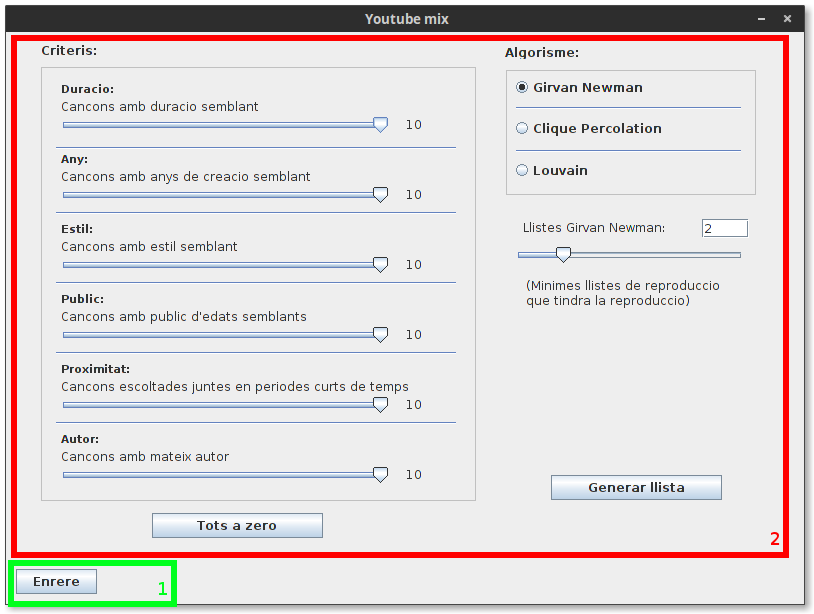
\includegraphics{interficie.png}

Youtube Mix te una interficie basica molt senzilla i intuitiva.
La finestra es compon de dues parts bàsiques, la zona de secció i el botó universal de tonar enrere.
\begin{enumerate}
\item {} 
\textbf{Enrere:} Aquest botó es troba present a totes les pàgines, i torna a la ultima pàgina consultada. Es possible que en certes pàgines, al presionar el botó de tornar enrere es demani confirmació. Això es degut a que es troba en una pàgina on s'introdueix o edita informació, i el fet de tornar enrere significa que aquesta informació es perdrà a no ser que sigui desada.

\item {} 
\textbf{La zona de secció:} Cada apartat del programa disposa d'una finestra pròpa de secció. Aquí es on res realitzen totes les funcions per interactuar amb el programa. Es pot trobar informació mes detallada sobre cada finestra de secció especifica en el seu apartat del manual.

\end{enumerate}


\chapter{Gestió d'usuaris}
\label{gest_usuaris::doc}\label{gest_usuaris:gestio-d-usuaris}
Es pot accecir a l'apartat de gestió d'usuaris presionant en ``Gestionar Usuaris'' de la finestra principal.


\section{Descripció de la interficie}
\label{gest_usuaris:descripcio-de-la-interficie}
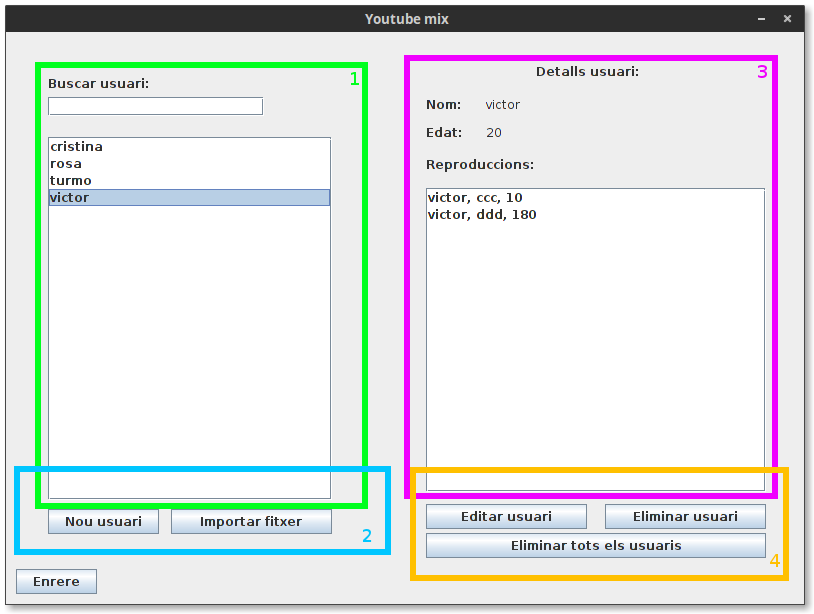
\includegraphics{gest_usr.png}
\begin{enumerate}
\item {} 
\textbf{Llista d'usuaris:} Seleccionant un usuari d'aquesta llista es pot consultar la seva informació. La informació i resproduccions de l'usuari seleccionat es mostraran a \textbf{l'apartat d'informació de l'usuari(3)}. També es disposa d'una barra d cerca per tal de buscar l'usuari desitjat.

\item {} 
\textbf{Introducció d'usuaris:} Es poden introduir els usuaris de dues formes diferents: Individualment (Introduint un nom i una edat) o important usuaris des d'un fitxer. Per informació sobre el format del fitxer, cansultar l'apartat ``Format del fitxer d'usuaris''.

\end{enumerate}

\begin{notice}{note}{Nota:}
En nom d'usuari es informació basica per a identificar l'usuari, i com a tal no pot ser modificat, asseguri's de que es correcte abans de desar el nou usuari.
\end{notice}
\begin{enumerate}
\setcounter{enumi}{2}
\item {} 
\textbf{Informació sobre l'usuari seleccionat:} En aquest apartat es mostra informació sobre l'usuari seleccionat. Nom, edat i cançons reproduides.

\item {} 
\textbf{Edició dels usuaris:} En aquest apartat es mostren les eines per a editar o eliminar els usuaris. Es pot eliminar un usuari individualment o be eliminar a tots els usuaris de cop. Editar usuari permet cambiar la edat d'un usuari així com gestionar les seves reproduccions. Consultar l'apartat ``Afegir reproduccions a un usuari'' per a mes informació sobre com gestionar les reproduccions d'un usuari.

\end{enumerate}


\section{Format del fitxer d'usuaris}
\label{gest_usuaris:format-del-fitxer-d-usuaris}
Per tal de poder importar un fitxer d'usuaris, el fitxer ha de seguir un format concret:

\begin{Verbatim}[commandchars=\\\{\}]
nom d\PYGZsq{}usuari;edat
\end{Verbatim}
\begin{itemize}
\item {} 
Un usari per linia.

\item {} 
Un nom d'usuari i una edat separat per '';'' i sense espais.

\item {} 
Si un usuari conté error, no serà importat (Per exemple usuari repetit o edat no numerica).

\end{itemize}

\begin{notice}{note}{Nota:}
Asseguri's de que el fitxer d'usuaris no acaba en una linia en blanc, això provocarà que els usuaris no s'importin correctament.
\end{notice}


\section{Afegir reproduccions a un usuari}
\label{gest_usuaris:afegir-reproduccions-a-un-usuari}
A part d'editar la seva edat, al editar un usuari es poden genstionar les seves reproduccions.

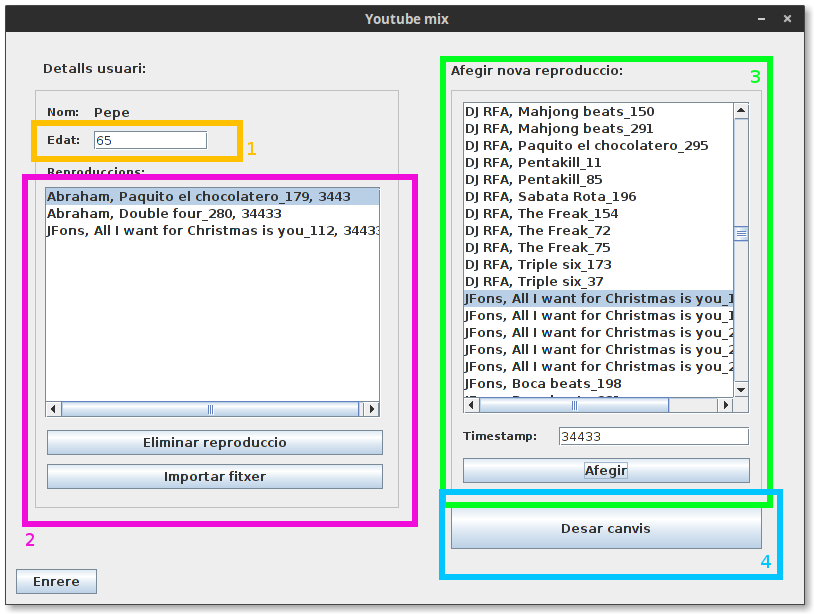
\includegraphics{edit_usr.png}
\begin{enumerate}
\item {} 
\textbf{Editar edat:} L'edat d'un usuari es editable, es pot cambiar aquí.

\item {} 
\textbf{Edició de reproduccions:} Aquí es poden veure les reproduccions d'un usuari, seleccionant una reproducció i presionant ``Eliminar reproducció'', eliminarà la reproducció seleccionada. També tenim la opció d'afegir reproduccions, importantlos d'un fitxer (consultar l'apartat ``Format del fitxer de reproduccions'' per mes informació sobre el format del fitxer) o individualment usant el \textbf{selector de cançons (3)} .

\end{enumerate}

\begin{notice}{note}{Nota:}
Si es desitja eliminar mes d'una reproducció, es pot presionar ctrl i seleccionar les reproduccions que desitgem eliminar.
\end{notice}
\begin{enumerate}
\setcounter{enumi}{2}
\item {} 
\textbf{Selector de cançons:} Es mostren les cançons disponibles al programa. Seleccionant una cançó de les disponibles i un timestamp, podem afegir la cançó com a escoltada per a l'usuari.

\item {} 
\textbf{Desar canvis:} Qualsevol canvi fet al usuari no serà aplicat fins a desarlos. Si es torna enrere sense desar els canvis, es perdran les modificacions.

\end{enumerate}


\section{Format del fitxer de reproduccions}
\label{gest_usuaris:format-del-fitxer-de-reproduccions}
Per tal de poder importar un fitxer d'usuaris, el fitxer ha de seguir un format concret:

\begin{Verbatim}[commandchars=\\\{\}]
\PYG{n}{Autor}\PYG{p}{;}\PYG{n}{titol}\PYG{p}{;}\PYG{n}{timestamp}
\end{Verbatim}
\begin{itemize}
\item {} 
Una reproducció per linia.

\item {} 
Camps separats per '';'' i sense espais.

\item {} 
Si una reproducció conté un error, no s'importarà  .

\end{itemize}

\begin{notice}{note}{Nota:}
Asseguri's de que el fitxer de reproduccions no acaba en una linia en blanc, això provocarà que les reproduccions no s'importin correctament.
\end{notice}


\chapter{Gestió de cançons}
\label{gest_cancons:gestio-de-cancons}\label{gest_cancons::doc}
Es pot accecir a l'apartat de gestió de cançons presionant en ``Gestionar Cançons'' de la finestra principal.


\section{Descripció de la interficie}
\label{gest_cancons:descripcio-de-la-interficie}
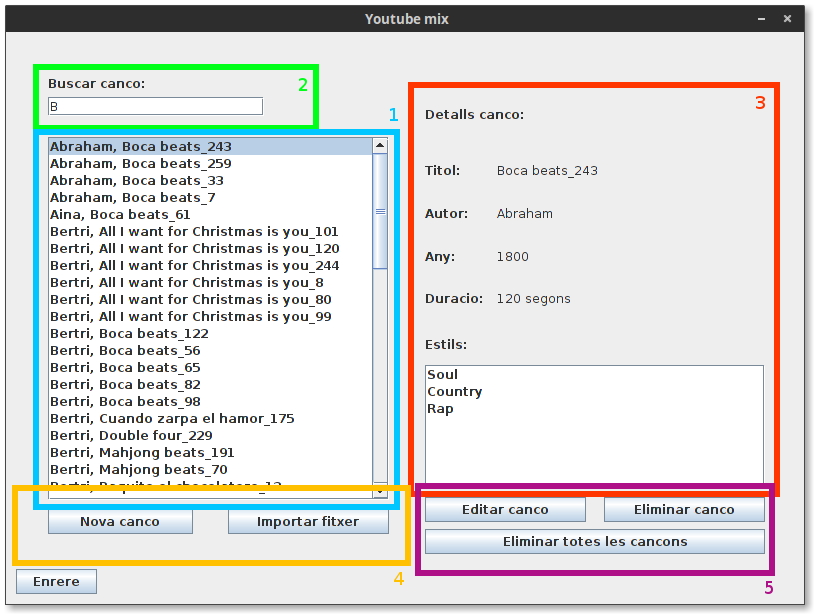
\includegraphics{gest_canco.png}
\begin{enumerate}
\item {} 
\textbf{Llista de Cançons disponibles:} En aquest apartat es poden consultar totes les cançons disponibles al programa, si la llista es molt gran, es pot usar \textbf{el buscador (2)} per filtrar les cançons i trobar la desitjada, al seleccionar una canço en aquesta llista, es podrà veure la seva informació en la \textbf{finestra de consulta d'informació (3)}.

\item {} 
\textbf{Buscador:} Introdueixio part del nom d'una cançó o un autor per filtrar el resultat.

\item {} 
\textbf{Consulta d'informació:} En aquest apartat es mostra la informació de la cançó seleccionada.

\item {} 
\textbf{Afegir cançons:} El programa disposa de dues formes d'introduir cançons noves, individualment o a partir d'un fitxer de cançons.
\begin{quote}
\begin{itemize}
\item {} 
\textbf{Introducció manual:} Presionant el botó ``Nova cançó'', s'accedirà a la introducció manual de cançons, La informació necesaria per a la introducció de la cançó es el nom de l'autor, el titol de la cançó, la duració en segons, l'any de publicació de la cançó i entre un i tres estils dels que la cançó formi part.

\end{itemize}

\begin{notice}{note}{Nota:}
Tant el titol com el nom de l'autor de la cançó son informació bàsica per identificar la cançó, i com a tal no pot ser modificada mes endavant, comprovi que sigui correcte abans de desar la informació.
\end{notice}
\begin{itemize}
\item {} 
\textbf{Importar d'un fitxer:} Es poden importar cançons a partir d'un fitxer, referirse a l'apartat ``Format del fitxer de cançons'' per una descripció del format que ha de tenir aquest fitxer.

\end{itemize}
\end{quote}

\item {} 
\textbf{Edició de les cançons:} En aques apartat es mostren les eines necessaries per editar i eliminar cançons, existeixen dues formes d'eliminar cançons, individualment o de forma massiva. Presionar a ``Eliminar totes les cançons'' elimina totes les cançons presents al programa. També es dona la opció de modificar la informació d'una cançó. Si us plau, referirse a la nota de l'apartat de introducció manual per a informació sobre el nom i l'autor de la cançó.

\end{enumerate}


\section{Format del fitxer de cançons}
\label{gest_cancons:format-del-fitxer-de-cancons}
Per tal de poder importar un fitxer de cançons, el fitxer ha de seguir un format concret:

\begin{Verbatim}[commandchars=\\\{\}]
Nom Artista;Titol Cançó;any;Estil 1;Estil 2;Estil 3;Duració en segons;
\end{Verbatim}
\begin{itemize}
\item {} 
Una cançó per linia, acabada en '';''.

\item {} 
Cada apartat ha d'anar separat amb '';'' i sense espais (o els espais seran interpretats com a part del camp).

\item {} 
Si la cançó no te 3 estils, es pot substituir Estil 2 i Estil 3 per ``-''.

\item {} 
Si existeix algun error en el format d'una cançó (Falta Estil 1, l'any o la duració no son numeros...), la cançó no s'importarà.

\end{itemize}

\begin{notice}{note}{Nota:}
Asseguri's de que el fitxer de cançons no acaba en una linia en blanc, això provocarà que les cançons no s'importin correctament.
\end{notice}


\chapter{Generació de llistes}
\label{gen_llistes:generacio-de-llistes}\label{gen_llistes::doc}
Es pot accecir a l'apartat de generació de llistes presionant en ``Generar llistes'' de la finestra principal.


\section{Descripció de la interficie}
\label{gen_llistes:descripcio-de-la-interficie}
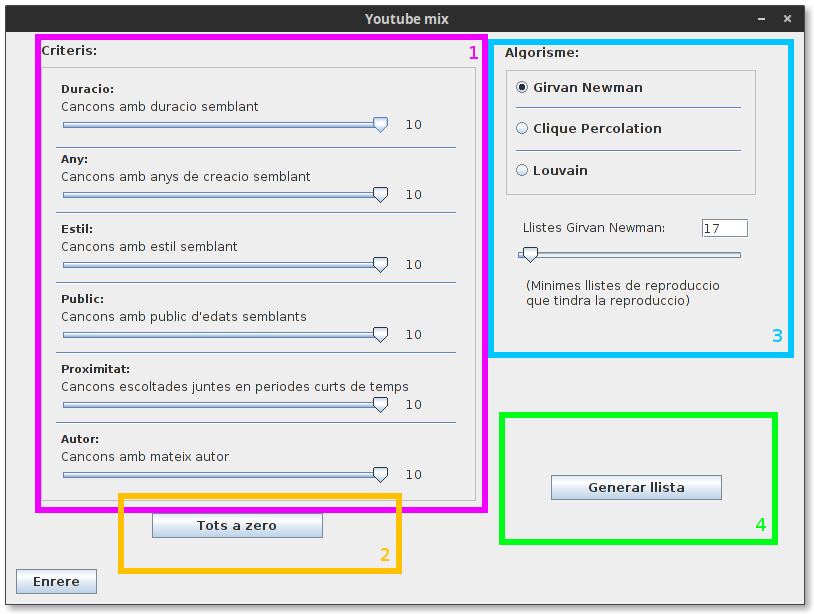
\includegraphics{gen_llist.png}
\begin{enumerate}
\item {} 
\textbf{Selector de ponderacions:} Usant els selectors d'aquest apartat, es poden seleccionar el valor de les ponderacions que s'usaran per generar les llistes. Cada un dels valor es troba explicat en eel selector, i son els seguents
\begin{itemize}
\item {} 
\textbf{Duració:} Les llistes es generaran tenint en compte la duració de la cançó. Cançons amb duracions semblants es trobaran en les mateixes llistes.

\item {} 
\textbf{Any:} Les llistes es generaran tenint en compte l'any en la que es va publicar la cançó. Cançons en anys pròxims es trobaran en les mateixes llistes.

\item {} 
\textbf{Estil:} Les llistes es generaran tenint en compte els seus estils. Cançons del mateix estil es trobaran en la mateixa llista.

\item {} 
\textbf{Public:} Les llistes es generaran tinguen en compte el public que acostuma a escoltarles. Si dues cançons les escolta gent d'edat semblant aniran a la mateixa lllista.

\item {} 
\textbf{Proximitat:}  Les llistes es generan tenint en compte cançons que s escolten normalment juntes. Dues cançons escoltades normalment juntes en un curt periode de temps pels usuaris aniran el les mateixes llistes.

\item {} 
\textbf{Autor:} Les llistes es generaran tenint en compte l'autor de les cançons. Dues cançons del mateix autor aniran a la mateixa llista.

\end{itemize}

\item {} 
\textbf{Tots a zero:} Si es vol resaltar un sol criteri, pot ser interssant posar tots els criteris a zero facilment per tan de que sigui mes ràpid seleccionar el desitjat.

\item {} 
\textbf{Selecció de l'Algorisme:} El programa disposa de 3 algorismes entre els que triar per tal de generar les llistes, amb aquest selector es pot indicar quin algorisme s'ha d'usar.

\end{enumerate}

\begin{notice}{note}{Nota:}
L'algorisme Girvan Newman permet també indicar el nombre minim de llistes que es generaran, seleccionant ``Girvan Newman'' apareixarà un selector per tal de triar aquest valor. Els valors disponibles depenen del nombre de cançons que hi hagi en aquell moment al programa.
\end{notice}
\begin{enumerate}
\setcounter{enumi}{3}
\item {} 
\textbf{Generar llista:} Al presionar aques botó, es generaran les llistes amb els criteris desitjats. Si us plau, tingui paciencia, ja que depenent de l'algorisme i el nombre de cançons, aquest procés pot trigar bastant.

\end{enumerate}


\section{Edició d'una solució generada}
\label{gen_llistes:edicio-d-una-solucio-generada}
Un cop generades les llistes, es poden editar per realitzar els canvis desitjats en aquest apartat.

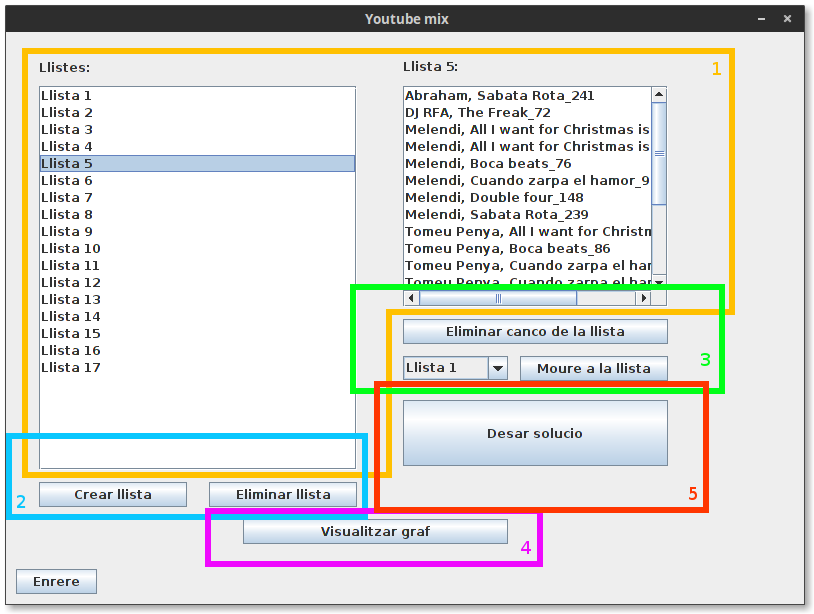
\includegraphics{edit_llist.png}
\begin{enumerate}
\item {} 
\textbf{Consulta de la solució:} En aquests apartats de la finestra es poden veure les diferents llistes generades. Seleccionant una de les llistes, es mostrarà al quadre de la dreta les cançons de les que esta formada.

\item {} 
\textbf{Edició de llistes:} Seleccionant una llista es pot eliminar presionant el botó de ``Eliminar llista''. Addicionalment, es poden afegir llistes buides a la solució per tal de mourehi cançons que es trobin a altres llistes.

\item {} 
\textbf{Edició de cançons:} Seleccionant una cançó d'una llista, es pot eliminar la cançó seleccionada de la llista, també existeix la opció de moure la cançó a una altre llista. Per a fer això, selecciona la nova llista de les disponibles en el menú i presiona ``Moure a la llista''.

\item {} 
\textbf{Visualitzar el graf:} Presionant en aquesta opció es pot consultar el graf de la solució. Per a mes informació, consultar l'apartat ``Consulta del graf''.

\item {} 
\textbf{Desar la solució:} Es desaran les llistes que hem modificat al gust per a futura consulta. Aquestes llistes estan disponibles al historial.

\end{enumerate}

\begin{notice}{note}{Nota:}
Les llistes un cop desades no poden ser modificades. Realitzi totes les edicións desitjades abans de desarla.
\end{notice}


\section{Consulta del graf}
\label{gen_llistes:consulta-del-graf}
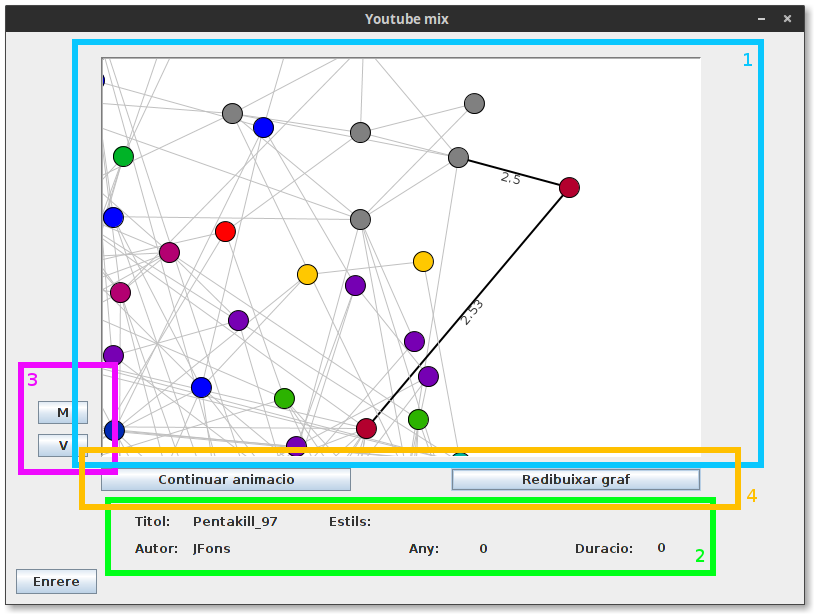
\includegraphics{consult_graf.png}

1. \textbf{Visualitxació del graf:} En aquesta finestra es mostra el graf de la solució. Cada llista de reproducció te les seves cançons (Nodes) d'un color diferent. Els nodes que apareixen ``transparent'' son cançons que no es troben a la solució final. Això pot ser degut a que s'han eliminat manualment, eren en una llista que ha sigut eliminada o que l'algorisme l'ha eliminat com a part del seu procés de generació.
Per a facilitar la consulta del graf, existeixen varies eines per moure's per la vista.
\begin{itemize}
\item {} 
\textbf{Clicar i arrossegar:} Permet moure's per el graf.

\item {} 
\textbf{La roda del ratolí:} Permer fer zoom per veure amb mes detall zones concretes del graf.

\item {} 
\textbf{Presionar shift mentre es clica i s'arrossega:} Permet girar el graf.

\item {} 
\textbf{Presionar ctrl mentre es clica i s'arrossega:} Permet sesgar el graf per consultarlo des de una prespectiva diferent.

\end{itemize}
\begin{enumerate}
\setcounter{enumi}{1}
\item {} 
\textbf{Informació sobre la cançó:} Al seleccionar un dels nodes amb el click esquerra del ratolí podem observar que s'activen dues funcions, primer de tot es pot consultar informació sobre la cançó seleccionada, que apareixerà en els espais per a text de sota del graf. També podem veure que els vertex (Les relacions amb altres cançons) de la cançó seleccionada es resalten, i es mostren les seves ponderacions.

\item {} 
\textbf{Mode Veure i mode moure:} Mab aquests botons es pot cambiar entre el mode veure (V) i el mode moure(M). El comportament descrit al punt 1 es el corresponent al mode Veure, que es el mode per defecte. Al seleccionar el mode Moure, podem clicar un o mes nodes (Clicant i arrossegant de forma que els nodes quedin inclosos en el rectangle que apareix) i es podem moure. aquesta funció es util si tenim un graf tan poblar pue es dificil llegir el seu contingut o les seves relacions i les volem apartar.

\item {} 
\textbf{Control de la vista del graf:} Per dibuixar el graf, el programa usa uns algorismes que apliquen forces als seus vertex i nodes a partir d'una posició aleatoria inicial. Amb ``Redibuixar graf'' tornem a posicionar aleatoriament els nodes i aplicar l'algorisme. Obtenint una nova distribució del graf. Amb aturar/continuar animació, podem pausar i continuar la animació dels vertex sen efectats per aquestes forces.

\end{enumerate}

\begin{notice}{note}{Nota:}
Obtenir un bon posicionament del graf es un problema molt complicat, per tant es molt possible que en grafs grans quedi tot molt junt i sigui dificil de llegir. Això es una limitació de l'algorisme i la velocitat del ordinador, i es dificil millorar el seu posicionament.
\end{notice}


\chapter{Consultar l'historial}
\label{consult_hist:consultar-l-historial}\label{consult_hist::doc}
Es pot accecir a l'historial presionant en ``Historial'' de la finestra principal.
Al historial es poden consultar totes les solucions generades que s'hagin desat.


\section{Descripció de la interficie}
\label{consult_hist:descripcio-de-la-interficie}
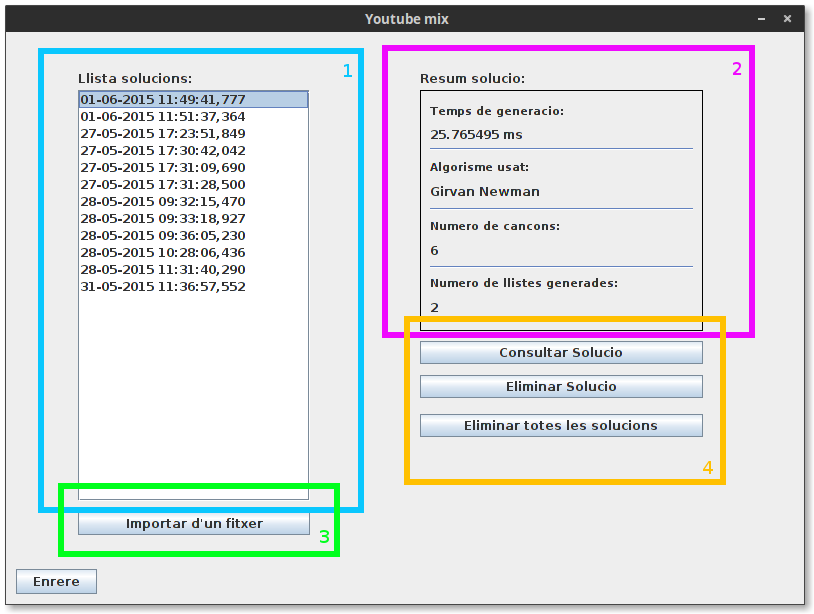
\includegraphics{consult_sol.png}
\begin{enumerate}
\item {} 
\textbf{Llistat de solucions desades:} Aquesta llista conté totes solucions que s'hagin desat, Al seleccionar una, es pot veure el seu resúm a l'espai de la dreta.

\item {} 
\textbf{Resúm de la solució:} En aquest apartat es mostra un resum de la solució seleccionada, per ajudar a identificarla. Es pot veure l'algorisme usat, el nombre de cançons i llistes generades, i el temps que ha trigat en generarse la solució.

\item {} 
\textbf{Importar solució d'un fitxer:} Es poden importar noves solucions que estiguin desades en un fitxerm per informació sobre el format d'una solució, consultat l'apartat ``Format d'un fitxer de solució''

\item {} 
\textbf{Eines d'edició de solucions:} en aquest apartat es mostren eines per gestionar i consultar les solucions, es pot eliminar la solució seleccionada o totes les solucions disponibles. També es pot consultar en detall la solució i el graf de la solució. Per mes informació sobre com funciona el visualitzador de graf, consultar l'apartat ``Consulta del Graf'' de la secció ``Generació de llistes''.

\end{enumerate}


\section{Format d'un fitxer de solució}
\label{consult_hist:format-d-un-fitxer-de-solucio}
El format de les solucions es complex, ja que ha de ser una capteta que contingui 3 documents i no està pensat per escriure manualment si no mes aviat per portar solucions generades pel programa a una altre copia del programa.

Una solució esta formada per una carpeta amb 3 document:
\begin{itemize}
\item {} 
\textbf{entrada.txt:} Aquest document desa una copia del graf d'entrada en un format que el programa pot interpretar per poguerlo consultar al consultar una solució desada.

\item {} 
\textbf{comunitats.txt:} En aquest document es la solució en si. Conté les diferents llistes de reproducció i les cançons per les que estan formades.

\item {} 
\textbf{info.txt:} En aquest document es desen informacions variades sobre la solució: L'algorisme usat, el temps de generació, el nombre de cançons i el nombre de llistes generades.

\end{itemize}


\chapter{Consultar les estadistiques}
\label{consult_estad:consultar-les-estadistiques}\label{consult_estad::doc}
En aquest apartat es poden consultar les estadistiques dels diferents algorismes. Es pot accedir pulsant ``Estadistiques'' a la finestra principal.


\section{Descripció de la interficie}
\label{consult_estad:descripcio-de-la-interficie}
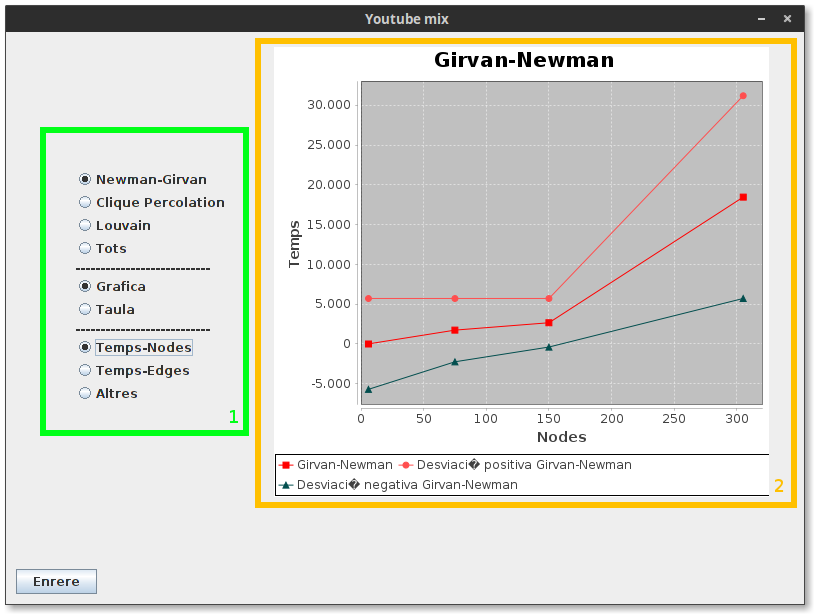
\includegraphics{consult_est.png}
\begin{enumerate}
\item {} 
\textbf{Selector del tipus d'estadistica:} Usant aquest selector, podem triar quina de les estadistiques volem consultar. Es poden veure estadistiques concretes de cada algorisme o la comparativa entre els tres algorismes disponibles. També es pot seleccionar veure la estadística en vorma de gràfica o consultar els valors en forma de taula.

\item {} 
\textbf{Visualitzador de dades:} Aquí es mostren les dades que haguem seleccionat en el selector (1). Consultar l'apartat ``Exportant les gràfiques com a imatge'' per mes informació sobre les altres funcionalitats.

\end{enumerate}


\section{Exportant les gràfiques com a imatge}
\label{consult_estad:exportant-les-grafiques-com-a-imatge}
Si es desitja desar una gràfica en concret, es pot desar en forma d'imatge per consultarla mes endavant un cop hagi sigut modificada.

Si es fa click amb el botó dret sobre la gràfica tindrem la opció de desarla com a .png, .pdf o en format vectorial.
Addicionalment, seleccionant ``preferencies'' podem editar la gràfica per tal de deixarla al nostre gust abans de desarla com a imatge.



\renewcommand{\indexname}{Índex}
\printindex
\end{document}
